%************************
\subsection{Patchen von Modellen}
%************************
Neben dem semantischen Liften von Differenzen besteht die Möglichkeit einen Patch zu erstellen und auf ein anderes Modell anzuwenden.\\

Abbildung \ref{silift-tutorial_patching_scenario} zeigt ein typisches Szenario der Patch-Anwendung.

\begin{figure}[h!]
\centering
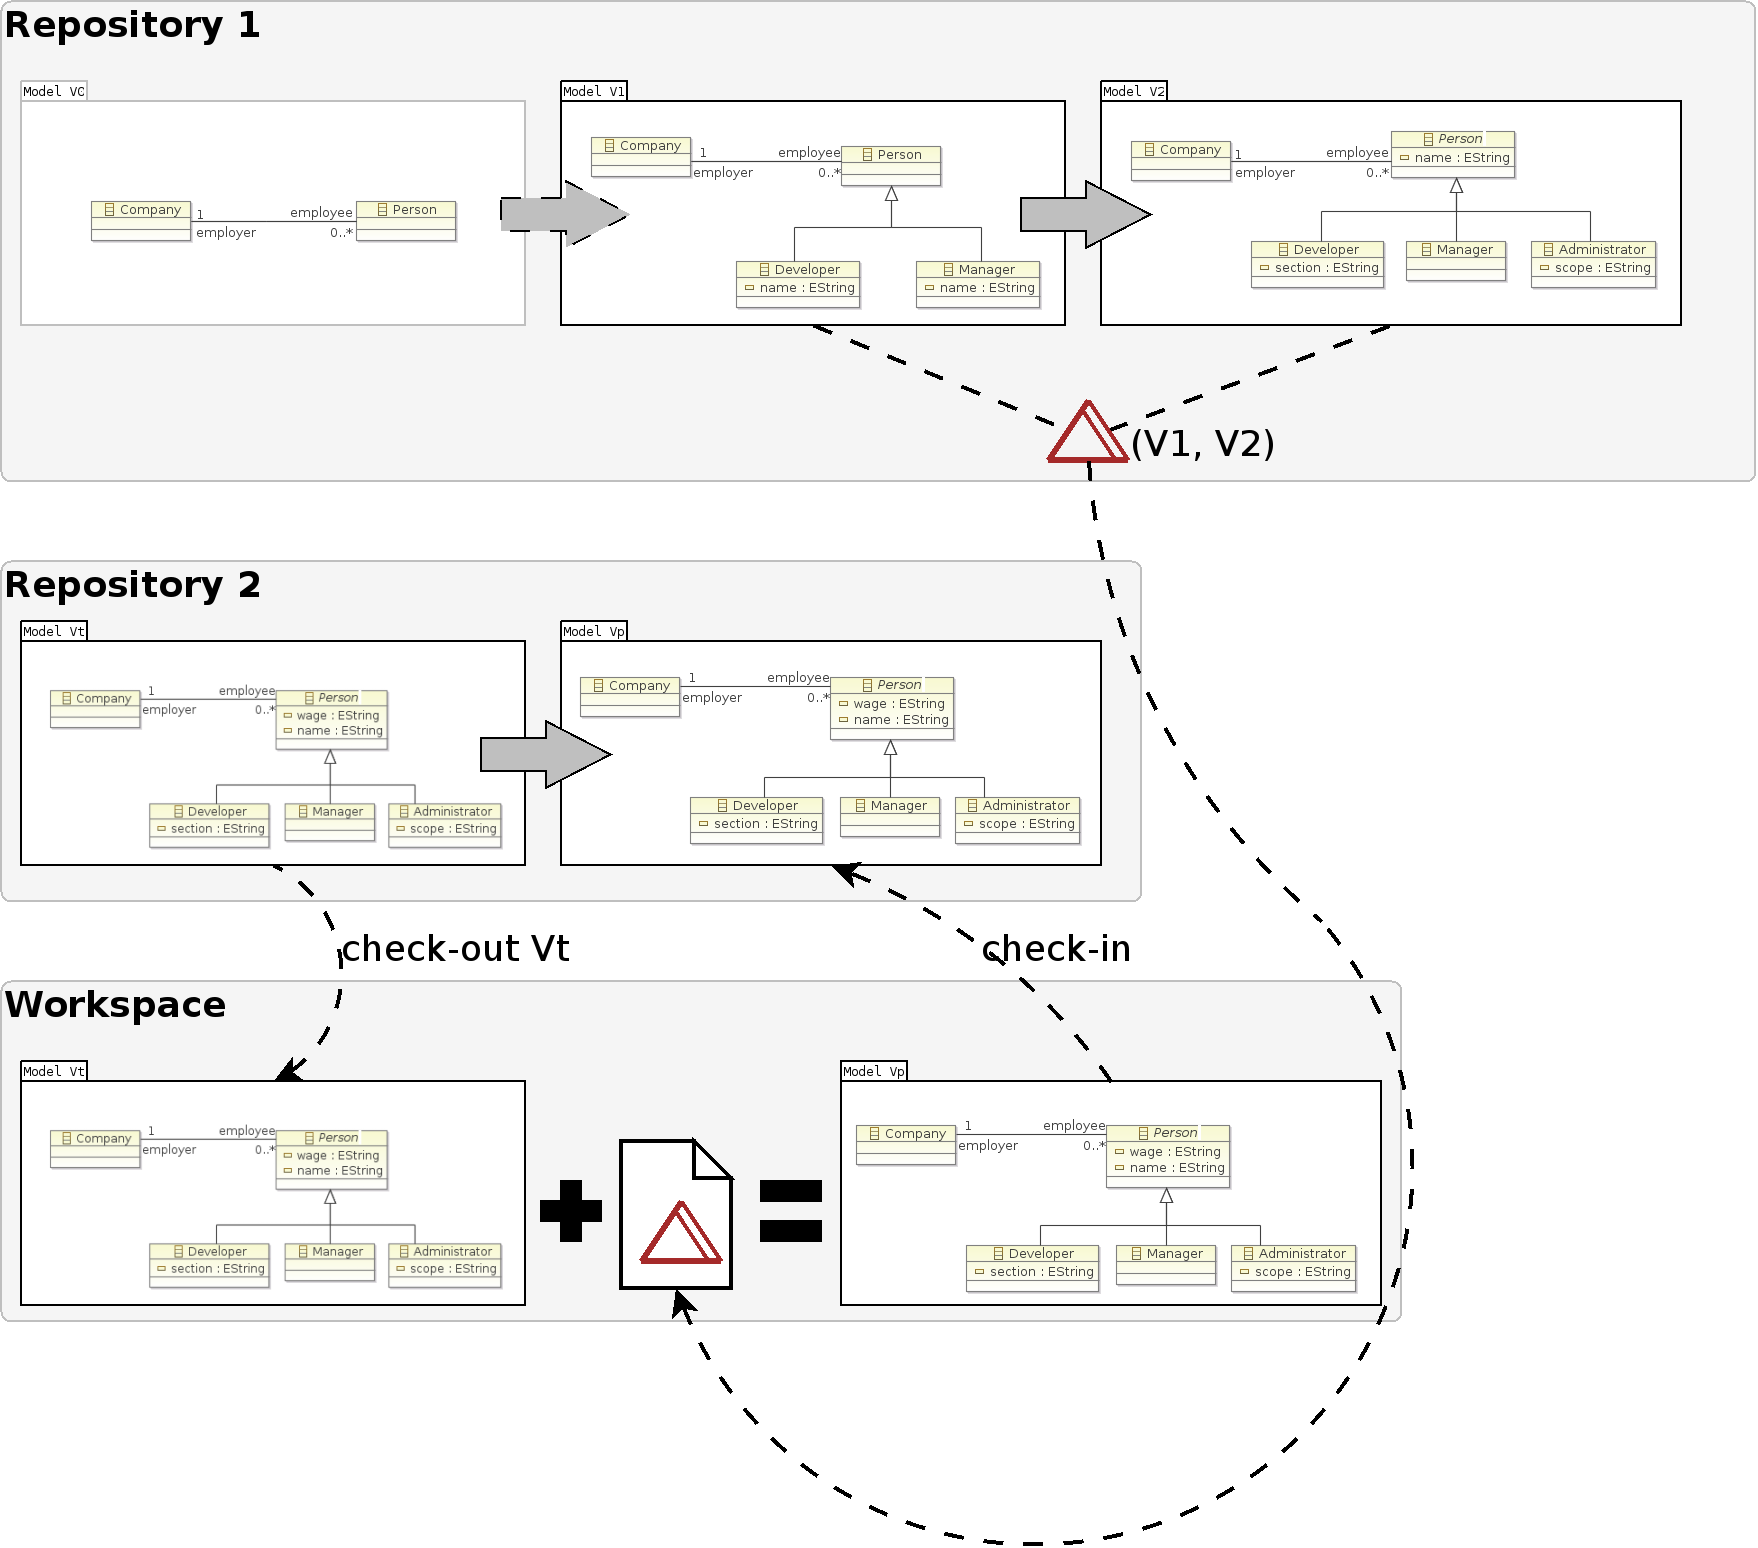
\includegraphics[width=\textwidth]{patching/graphics/silift-tutorial_patching_scenario.png}
\caption{Ablauf einer Patch-Anwendung}
\label{silift-tutorial_patching_scenario}
\end{figure}



\texttt{Repository 1} stellt den Entwichklungsprozess eines Modells dar, welches zu einem bestimmten Zeitpunkt (hier \texttt{Model V1}) in ein zweites Repository übertragen und dort ggf. weiterentwickelt wird (vgl. \ref{silift-tutorial_patching_scenario}, \texttt{Repository 2}, \texttt{Model Vt}).\footnote{\texttt{Model Vt} und \texttt{V1} bzw. \texttt{V2} können auch unabhängig von einander entwickelt worden sein.} 
Des Weiteren wird das Modell auch in \texttt{Repository 1} weiterentwickelt bzw. überarbeitet.
Dieses Refactoring soll nun auf \texttt{Model Vt} in \texttt{Repository 2} angewandt werden, ohne dass die bereits vorgenommenen Änderungen an diesem verloren gehen.
Zu diesem Zweck wird eine \textit{asymmetrische Differenz} zwischen \texttt{Model V1} und \texttt{Model V2} gebildet und in Form eines Patches auf \texttt{Model Vt} angewandt (vgl. \ref{silift-tutorial_patching_scenario}, \texttt{Workspace}).\\
Sofern in beiden Modellen Änderungen an dem gleichen Element vorgenommen wurden,  können einzelne Editieroperationen des Patches ggf. nicht mehr angewandt werden.\\

Im Folgendem lernen Sie, wie Sie mit Hilfe von SiLift einen Patch erstellen und auf ein ein Modell anwenden können.

\subsubsection{Erstellen eines Patches}

Um einen Patch zu erstllen selektieren Sie im Package bzw. Project Explorer die beiden Modelle zwischen denen die asymmetrische Differenz berechnet werden soll.
Öffnen Sie mit der rechten Maustaste das Kontextmenü und wählen Sie \texttt{SiLift} $\triangleright$ \texttt{Create a Patch} aus (vgl. Abb. \ref{silift-tutorial_patching_contextmenu_create}).

\begin{figure}[H]
\centering
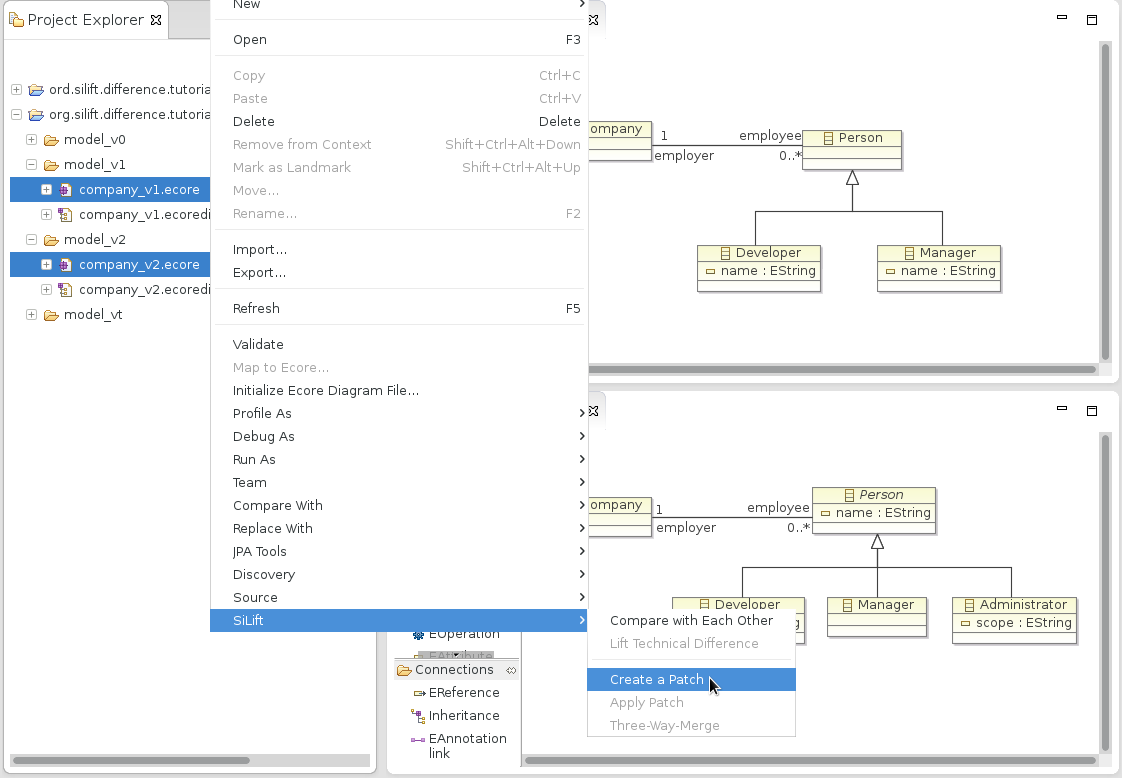
\includegraphics[width=0.8\textwidth]{patching/graphics/silift-tutorial_patching_contextmenu_create.png}
\caption{SiLift: Patch erstellen}
\label{silift-tutorial_patching_contextmenu_create}
\end{figure}

Es öffnet sich ein neues Fenster, welches analog zu Abbildung \ref{silift-wizard_compare_page1} mehrere Konfigurationsmöglichkeiten bietet (vgl. Abb. \ref{silift-tutorial_patching_create_config}).


\begin{figure}[H]
\centering
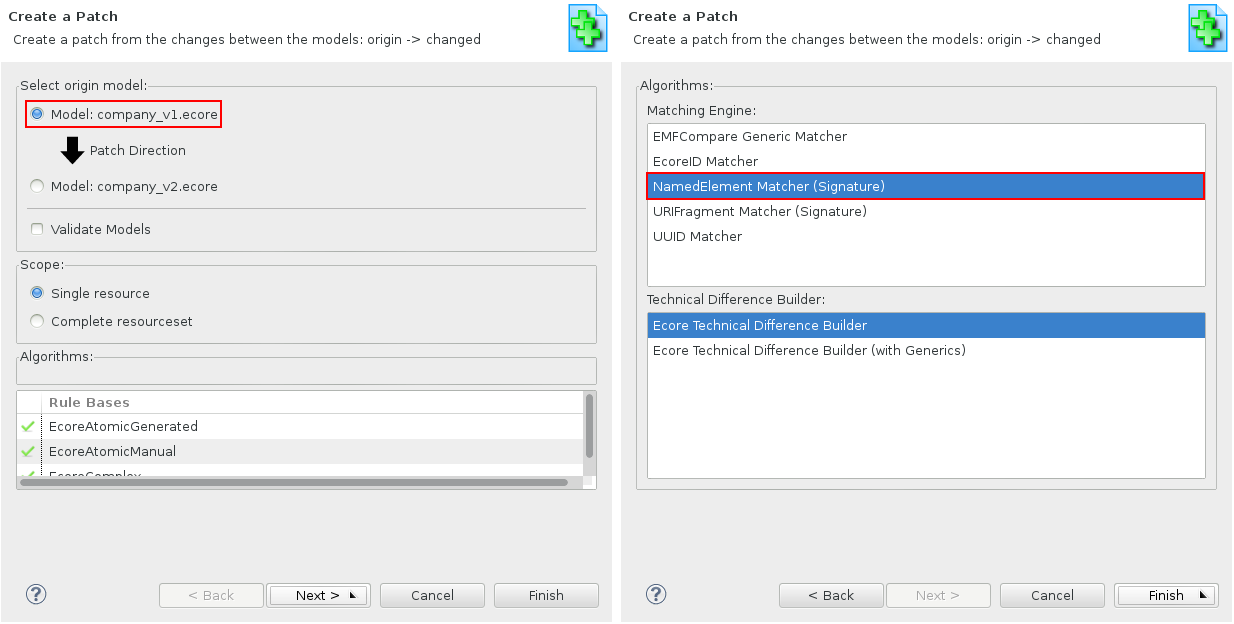
\includegraphics[width=0.8\textwidth]{patching/graphics/silift-tutorial_patching_create_config.png}
\caption{Patch-Config}
\label{silift-tutorial_patching_create_config}
\end{figure}

Nach erfolgreicher Generierung wird der Patch im Ordner des Basismodells gespeichert und in einem entsprechenden Editor geöffnent.
Dieser bietet die Möglichkeit einen Patch nachträglich noch zu bearbeiten, indem einzelne Editieroperationen deaktiviert werden können (vgl. Abb. \ref{silift-tutorial_patching_modify_patch}).

\begin{figure}[H]
\centering
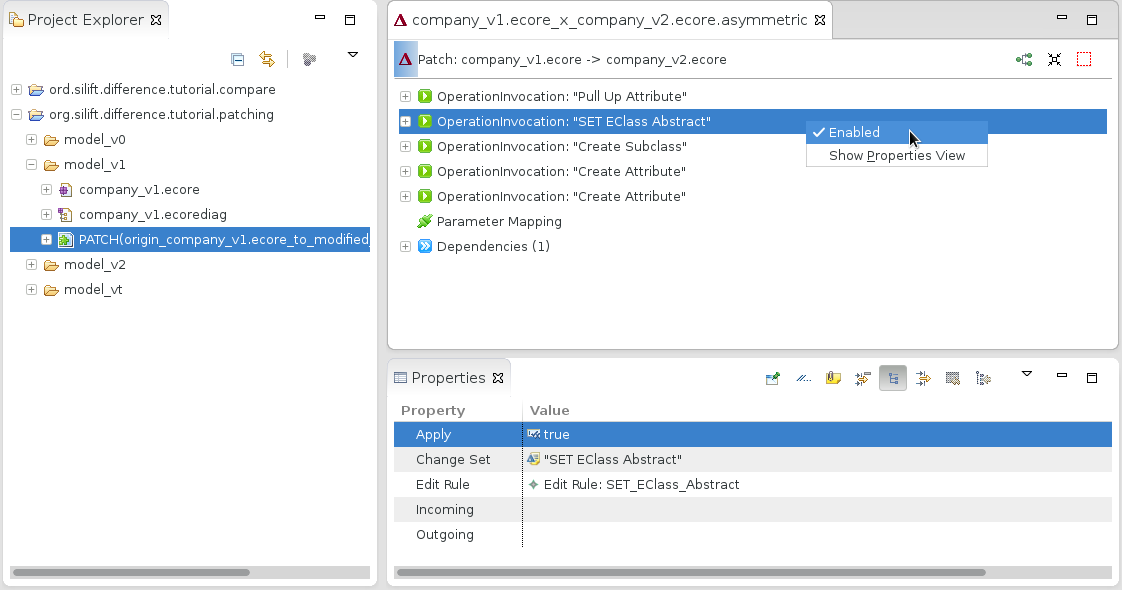
\includegraphics[width=0.8\textwidth]{patching/graphics/silift-tutorial_patching_modify_patch.png}
\caption{Patch-Editor}
\label{silift-tutorial_patching_modify_patch}
\end{figure}

\subsubsection{Anwenden eines Patches} \label{sec:patching_apply}

Das Anwenden eines Patches erfolgt wieder über das Kontextmenü von Eclipse.
Klicken Sie mit der rechten Maustaste auf den Patch im Package bzw. Project Explorer und wählen Sie \texttt{SiLift} $\triangleright$  \texttt{Apply Patch} aus (vgl. Abb. \ref{silift-tutorial_patching_contextmenu_apply}).

\begin{figure}[H]
\centering
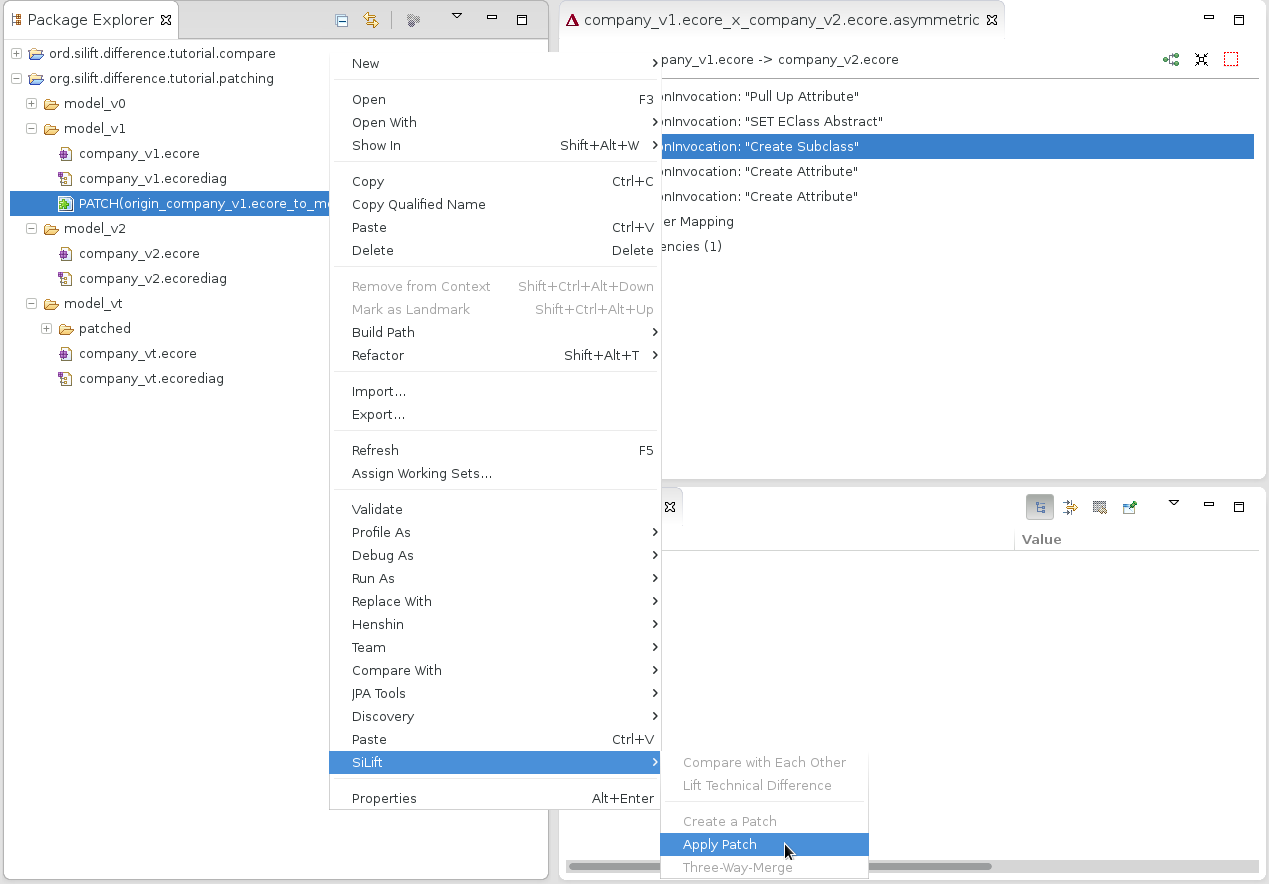
\includegraphics[width=0.8\textwidth]{patching/graphics/silift-tutorial_patching_contextmenu_apply.png}
\caption{SiLift: Patch anwenden}
\label{silift-tutorial_patching_contextmenu_apply}
\end{figure}

Es öffnet sich ein Dialogfenster, das sich in einigen Punkten von den zuvor beschriebenen unterscheidet.\\
Auf der ersten Seite muss zum einen das Zielmodell, auf welches der Patch angewandt werden soll, angegeben werden, zum anderen besteht die Mögichkeit zwischen verschiedenen Validierungsmodi zu wählen (vgl. \ref{silift-tutorial_patching_apply_config_page01}).
\texttt{Model Validation} prüft das Modell vor und nach einer Operationsausführung.
D.h. wenn mehrere Regeln automatisiert nacheinander ausgeführt werden, wird das Modell zwei mal überprüft.
\texttt{Iterative Validation} prüft hingegen das Modell nach jeder Operationsausführung.

\begin{figure}[H]
\centering
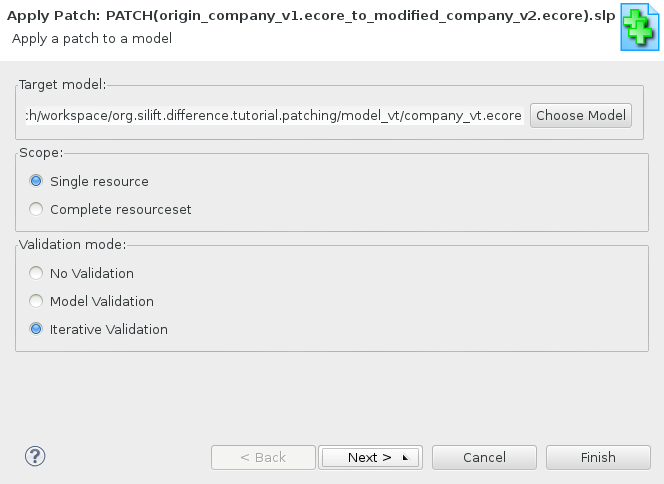
\includegraphics[width=0.6\textwidth]{patching/graphics/silift-tutorial_patching_apply_config_page01.png}
\caption{Einstellungen für das Anwenden eines Patches: Seite 1}
\label{silift-tutorial_patching_apply_config_page01}
\end{figure}

Analog zu dem Vergleichsdialog und dem zum Erstellen eines Patches, bietet die zweite Seite eine Liste von verfügbaren Matchern, aus der einer zu wählen ist.
Handelt es sich bei der Auswahl um einen ähnlichkeitsbasierten Matcher, so muss noch ein minimaler Verlässlichkeitswert angegeben werden (vgl. Abb. \ref{silift-tutorial_patching_apply_config_page02}).
Klicken Sie auf \texttt{Finish}.

\begin{figure}[H]
\centering
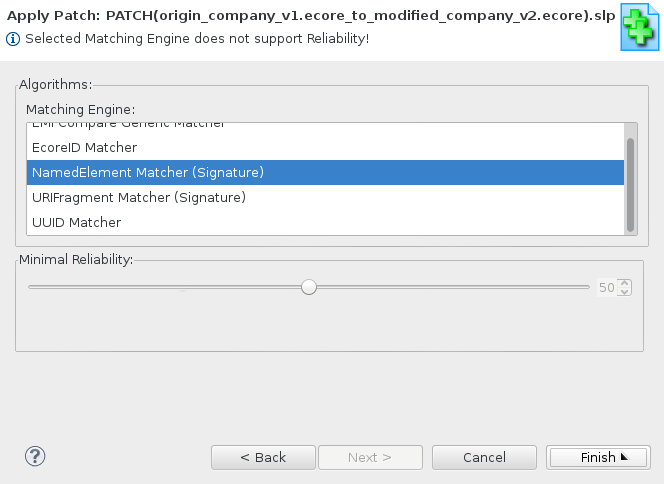
\includegraphics[width=0.6\textwidth]{patching/graphics/silift-tutorial_patching_apply_config_page02.png}
\caption{Einstellungen für das Anwenden eines Patches: Seite 2}
\label{silift-tutorial_patching_apply_config_page02}
\end{figure}

Es öffnet sich eine neue Perspektive bestehend aus einem Editor und drei Eclipse-Views, welche im Folgendem genauer betrachtet werden (vgl. Abb. \ref{silift-tutorial_patching_perspective}).

\begin{figure}[H]
\centering
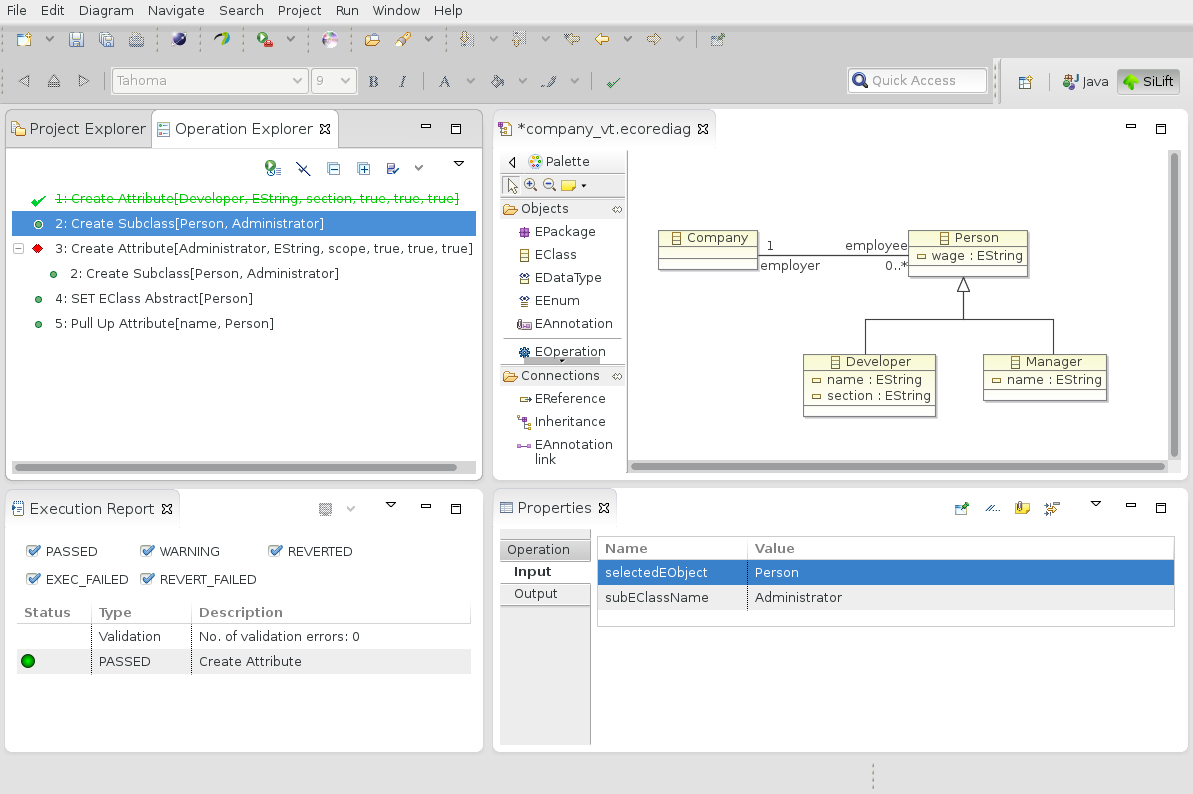
\includegraphics[width=0.8\textwidth]{patching/graphics/silift-tutorial_patching_perspective.png}
\caption{Patching Perspektive}
\label{silift-tutorial_patching_perspective}
\end{figure}

\paragraph{Operation Explorer}

Mit Hilfe des \textit{Operation Explorer} können die jeweiligen Operationen des Patches auf das Modell im \texttt{Editor} angewandt werden.

\begin{figure}[H]
\centering
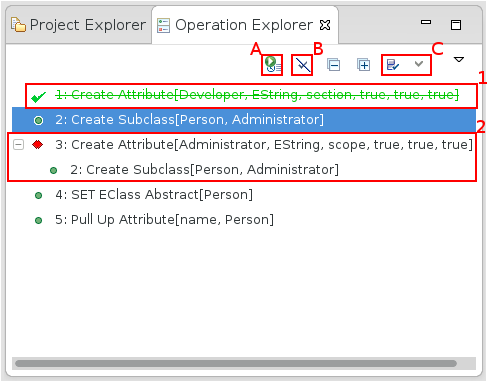
\includegraphics[width=0.6\textwidth]{patching/graphics/silift-tutorial_patching_operation_explorer.png}
\caption{Operation Explorer}
\label{silift-tutorial_patching_operation_explorer}
\end{figure}

\begin{enumerate}
	\item Bereits ausgeführte Operationen (grün) bzw. ignorierte Operationen (grau) (können durch \texttt{B} ausgeblendet werden).
	\item Abhängige Operationsausführungen: Eine Operationsausführung kann Abhängigkeiten zu anderen besitzen. So muss in unserem Beispiel die Klasse \texttt{Administrator} vor dem Attribut \texttt{scope} erzeugt werden.
\end{enumerate}

\begin{enumerate}[(A)]
	\item Führt alle konfliktfreien Operationen aus. Einzelne Operationen können durch Doppelklick oder Rechtsklick ausgeführt bzw. rückgängig gemacht werden (vgl. Abb. \ref{silift-tutorial_patching_operation_explorer_contextmenu}).
	\item Blendet alle bereits ausgeführten und/oder ignorierten Operationen ein bzw. aus. Operationen können über Rechtsklick von der Ausführung ausgeschlossen, also ignoriert werden (vgl. Abb. \ref{silift-tutorial_patching_operation_explorer_contextmenu}).
	\item Validierungsmodus wechseln.
\end{enumerate}

\begin{figure}[H]
\centering
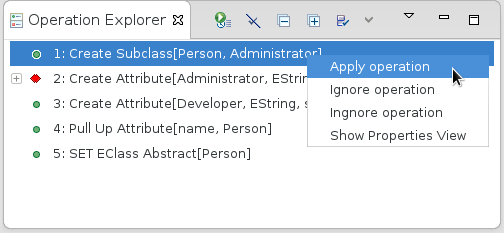
\includegraphics[width=0.6\textwidth]{patching/graphics/silift-tutorial_patching_operation_explorer_contextmenu.png}
\caption{Operation Explorer Kontextmenü}
\label{silift-tutorial_patching_operation_explorer_contextmenu}
\end{figure}

\paragraph{Properties}
Die \textit{Properties View} bietet zum einen allgemeine Informationen zu einer selektierten Operation, zum anderen besteht die Möglichkeit die Eingabeparameter einer Operation zu ändern (vgl. Abb. \ref{silift-tutorial_patching_properties_View}).

\begin{figure}[H]
\centering
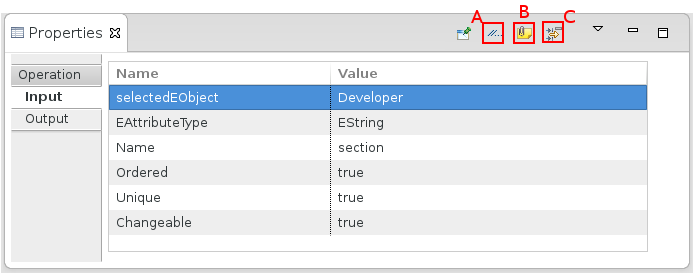
\includegraphics[width=0.8\textwidth]{patching/graphics/silift-tutorial_patching_properties_view.png}
\caption{Properties View}
\label{silift-tutorial_patching_properties_View}
\end{figure}

\begin{enumerate}[(A)]
	\item Aktivierung qualifizierter Bezeichner: Manchmal kommt es vor, dass einige Modellelemente (z.B. Attribute in unterschiedlichen Klassen) einen gleichen Bezeichner besitzen. Daher kann es hilfreich sein, sich den qualifizierten Bezeichner anzeigen zu lassen. Dieser setzt sich i.d.R. aus dem Bezeichner des Modellelements und denen der Container-Elemente zusammen.
	\item Anzeige des Verlässlichkeitswertes.
	\item Ein- bzw. ausblenden weiterer Attribute.
\end{enumerate}

\paragraph{Execution Report}
Der \textit{Execution Report} enthält Informationen über die zuletzt ausgeführte Operation. Diese Informationen umfassen zum einen den Status der Operationsausführung (\texttt{PASSED}, \texttt{WARNING} etc.), zum anderen, ob das resultierende Modell noch bzw. wieder valide ist (vgl. Abb. \ref{silift-tutorial_patching_execution_report}).

\begin{figure}[H]
\centering
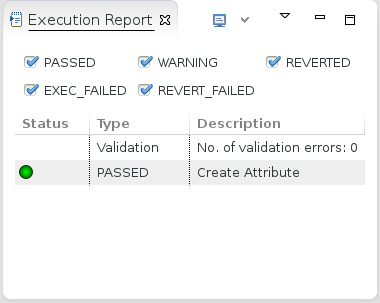
\includegraphics[width=0.6\textwidth]{patching/graphics/silift-tutorial_patching_execution_report.png}
\caption{Execution Report}
\label{silift-tutorial_patching_execution_report}
\end{figure}

Der angezeigte Report enthält nur Informationen über die zuletzt ausgeführte Operation. Sofern man Informationen zu den vorherigen Ausführungen einsehen möchte, kann man diese über den \textit{Report Stack} abrufen (vgl. Abb. \ref{silift-tutorial_patching_execution_report_stack}).

\begin{figure}[H]
\centering
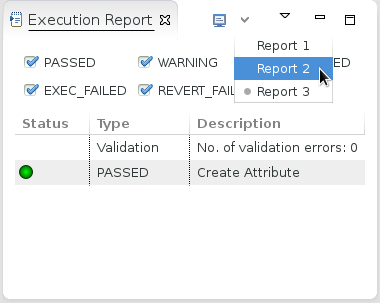
\includegraphics[width=0.6\textwidth]{patching/graphics/silift-tutorial_patching_execution_report_stack.png}
\caption{Report Stack}
\label{silift-tutorial_patching_execution_report_stack}
\end{figure}